From an junction temperature of -40\(\degree \)C to +175\(\degree \)C, the experimental measurements of the propagation delay pose an interesting challenge. Earlier works have used simple as well as complex circuits for delay extraction. 

The easiest solution would be to externalize the clock and the outputs of the comparator to extract the delay by a high speed high resolution measurement device. Unfortunately, outputs drivers consumes much chip area, add extra delay, bond-wires inductances would alter the signal and the delay estimation too, and different length of cables between the clock of reference and the output generates unconditional error prone measurement system.

For a simple solution of delay measurement, one can generates a DC voltage proportional to the delay. In the case of a clocked comparator, continuous decisions made are averaged by a low-pass filter to externalize a DC voltage. Difficulties occur as a pulse indicates a ``decision made'' event whose width is sensitive to the parasitics and PVT variations. While the PVT variations can be alleviated by the employ of mathematical expressions for differential output pulses as in~\cite{1706643}, it suffers of mismatch in parasitics seen by XOR cells within the pulse of reference generator and the generator of the ``decision made'' pulse.

For instance, high precision time interval measurement systems are commonly used in Telecommunications, nuclear science, frequency synthesis, measurement devices such as oscilloscopes and logic analyzers, and time-of-flight cameras are heavily relying on time-to-digital converters (TDC). In a nutshell, a TDC is made with a counter and delay line interpolation~\cite{1637593}. Such converters have a limited achievable accuracy in a technology based on the small delay cell (an inverter), the quantization noise, and the non-linearity in the time interpolation. The latter coming from variation in the delay elements of the smallest delay cell, as the cascade of delay cells increase, the integral non-linearity grows such that accurate measurement of large delay is challenging.

In contrast, measurement circuits based on Vernier delay line can achieve fine delay resolution.

% figure of practical implementations
\begin{figure}[htp]
    \centering
    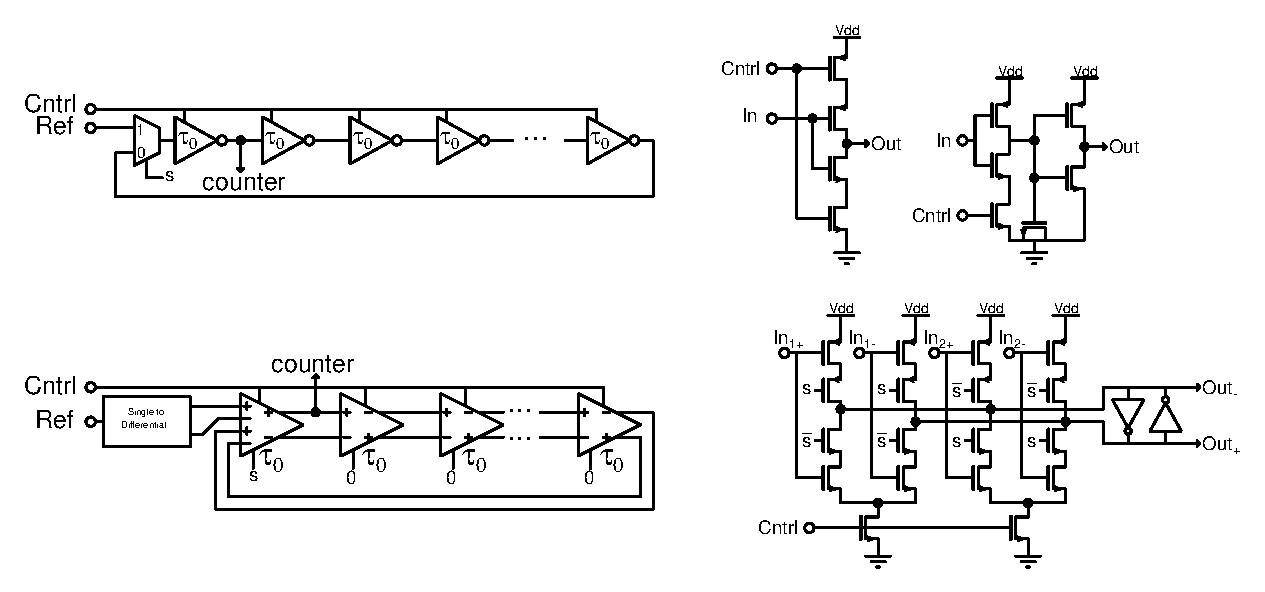
\includegraphics[width=\textwidth]{Chapter5/Figs/delay_line_implementation_possible.ps}
    \caption{Some delay line implementation for the delay estimation and practical implementations of delay cells}
    \label{fig:delay_vernier_interpolation}
\end{figure}

Practical implementations of the delay line and interpolation is depicted by \figurename~\ref{fig:delay_vernier_interpolation}. J.P. Jansson \textit{et al.} use the differential implementation represented in this figure. To estimate the delay a synchronous counter performs a coarse estimation of the delay while the recorded state of the delay line divides the clock of the counter into pieces of \(\Delta T\)~\cite{1637593}. The recorded state of the delay line corresponds to the value stored by DFFs of the positive output of these delay cells.

That said, averaging results either in the time domain or by several TDC running in parallel mitigates the non-linearity: the improvements being inversely proportional to the square root of measurements. However, they are sensitive to PVT variations~\cite{6233014, 5256168} such that calibration is mandatory. Finally, this method does not timely occupy a silicon footprint for built-in self-test.

Finally, the ring oscillator can also be employed to estimate the delay as in~\cite{8267856} wherein perused different oscillators related to the device under test can accurately calculate the delay of element under test. In the case of~\cite{8267856} the delay of Through-Silicon Via for 3D IC are measured. This solution fit within a small silicon area with a large measurement range. Unfortunately, as the number of oscillators increase, mismatch of their instance is averaged and the calculus of the delay becomes even more tedious. Furthermore, it is difficult from the design phase to estimate the accuracy of measurement.
\nomenclature[z]{IC}{Integrated Circuit}

\subsubsection{Delay measurement Principle}
Therefore, we proposed a circuit to reliably measure the comparator's delay with a differential measure of frequency generated by an auto-oscillator with an estimation of the measurement accuracy early in its design phase. The generated frequency is then divided by an arbitrary ratio N to be measured. It prevents high speed signal routing consideration.

The auto-oscillator generates a first frequency of reference without the comparator only based on digital cells. Then, with the same digital cells configuration the frequency is generated by fully restored comparator's outputs in response to the comparators input voltages when the frequency trigger the comparator.

% image of the layout to give the area
\begin{figure}[htp]
    \centering
    \begin{subfigure}[b]{0.47\linewidth}
	    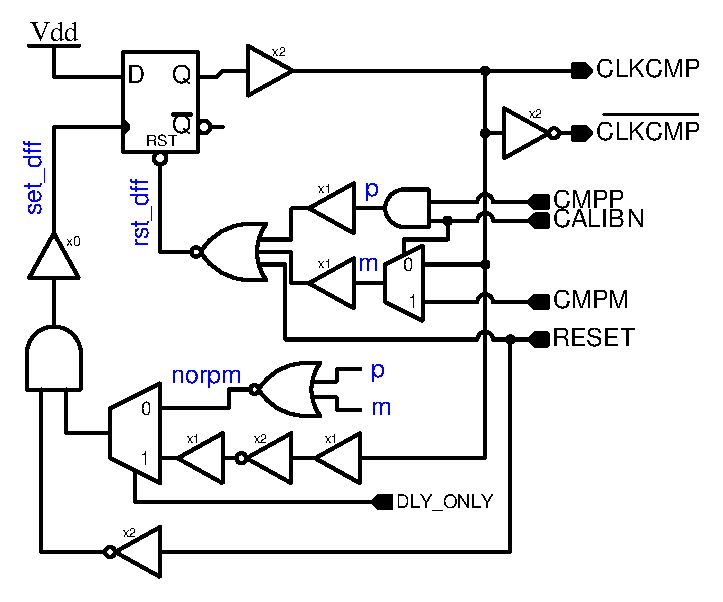
\includegraphics[width=\textwidth]{Chapter5/Figs/test_delay_comp_new_simp.ps}
    \end{subfigure}
    \begin{subfigure}[b]{0.50\linewidth}
	    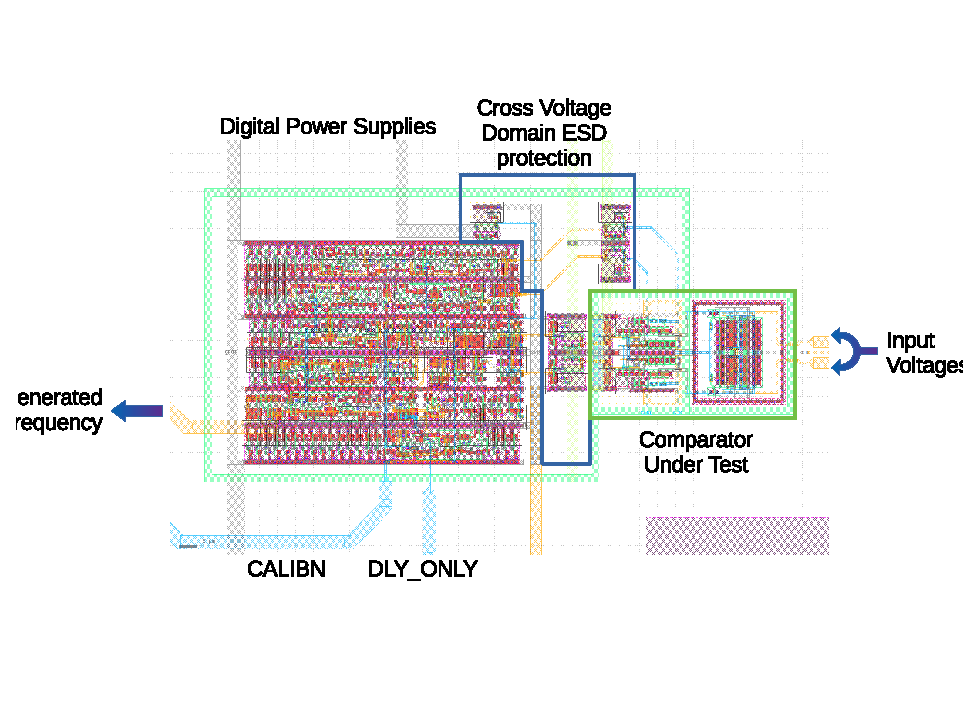
\includegraphics[width=\textwidth]{Chapter5/Figs/layout_delay_meas.eps}
    \end{subfigure}
    \caption{Schematic of the proposed measurement circuit and the delay test dimension}
	\label{fig:meas_circ_schem}
\end{figure}

\figurename~\ref{fig:meas_circ_schem} represents the auto-oscillator circuit connected to the comparator under test. Build around a central D-Flip-Flop generating our frequency CLKCMP, an inverter is used to generate the complementary clock with some delay (\(\approx\)70 ps) to test the Double-Tail comparator.

CALIBN signal allows us to choose the generated frequency: the frequency of reference or the frequency with the comparator to extract the delay. As the comparator requires some time to reset, the required time to reset can also be extracted. To select whether we need to extract only the delay or the delay and the reset time of the comparator DLY\_ONLY shall respectively be set to `1' and `0'. And the RESET signal sets the CLKCMP signal to `0' which in turn resets the comparator under test. To change from the generation of one frequency to another, a reset is necessary.

For the sake of clarity, we comply with the following frequency names for each configuration possible:
\begin{table}[htp]
    \centering
    \begin{tabular}{@{}ccc@{}}
    \toprule
    DLY\_ONLY & CALIBN & Frequency Name \\ \midrule
    1 & 0 & $F_{\rm CLKCMP1}$ \\
    1 & 1 & $F_{\rm CLKCMP2}$ \\
    0 & 0 & $F_{\rm CLKCMP3}$ \\
    0 & 1 & $F_{\rm CLKCMP4}$ \\ \bottomrule
    \end{tabular}
\end{table}

When the signal RESET is released, the reset signal of the DFF is disengaged and CLKCMP keep its state. Few picoseconds later, the clock signal of the DFF rises to `1'. This edge triggers the DFF which sets its outputs Q to `1', as depicted by the \figurename~\ref{fig:meas_circ_trans} a and b. In consequence, the comparator makes a decision. The DFF is triggered either by the nor of p and m signal if CALIBN is `1' or by the inversion of CLKCMP if CALIBN is `0'. The DFF is reset, and the oscillations begin.

For DLY\_ONLY set to `1', the clock of the DFF (set\_dff) is a delayed \(\overline{CLKCMP}\). Therefore, the time of CLKCMP spend at zero is fixed and PVT dependant. While, for a DLY\_ONLY signal set to `0', the signal set\_dff depends from the generated pulse of the nor gate. In that case, the time that CLKCMP spent at zero is defined by the speed of the comparator to reset.

The frequency difference between the two modes defined by CALIBN corresponds to the mismatch of the MUX inputs selecting either CMPM or CLKCMP, and the delay of the comparator to make a decision. While, the difference introduced by the two states of DLY\_ONLY corresponds to the difference of the delay and the time to reset the comparator. Thus, the proposed circuit is able to extract the delay of the comparator or the delay and the time to reset the comparator.

\begin{figure}[htp]
	\begin{minipage}[b]{0.47\linewidth}
	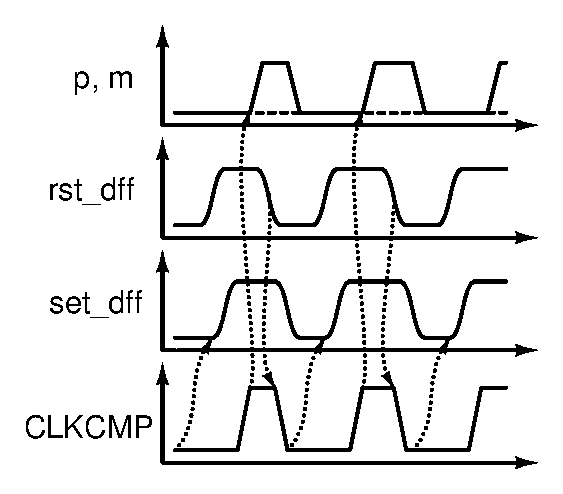
\includegraphics[width=\linewidth]{Chapter5/Figs/test_delay_comp_new_tare0_bypass1.ps}
	\subcaption{CALIBN='0'}
	\end{minipage}
	\begin{minipage}[b]{0.47\linewidth}
	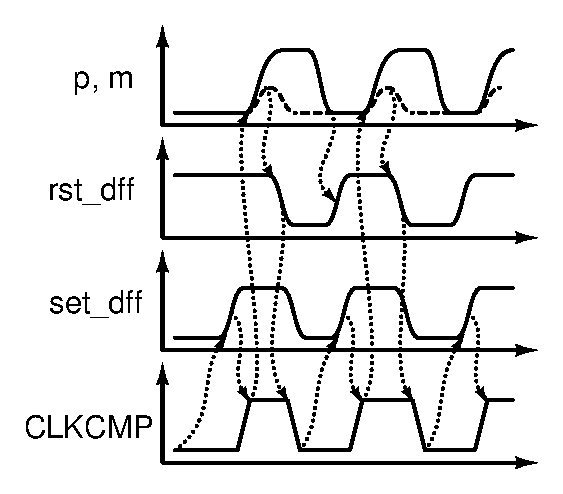
\includegraphics[width=\linewidth]{Chapter5/Figs/test_delay_comp_new_tare1_bypass1.ps}
	\subcaption{CALIBN='1'}
	\end{minipage}
	\caption{Measurement circuit transient behavior}
	\label{fig:meas_circ_trans}
	\vspace{-1em}
\end{figure}

As the same path is used for the generation of the frequency of reference and the frequency with the comparator under test, the PVT dependence of digital cells is the same in either generation case. Therefore, the differential measurement of the frequency cancels the PVT variations.

The calculation of the frequency in the normal operation mode (CALIBN='1' and DLY\_ONLY=RESET='0') is given by the equation (\ref{eqn:freq_meas_circuit_delay}).

\begin{equation} \label{eqn:freq_meas_circuit_delay}
F_{\rm CLKCMP4} = \frac{1}{N} {\left(T_{delay}+T_{set}+T_{rst}+T_{reset}\right)}^{-1}
\end{equation}

where $T_{delay}$ is the delay of the comparator, $T_{reset}$ the time the comparator takes to reset, and $T_{set}$/$T_{rst}$ the time of the digital circuit to react. In detail, $T_{set} = 2 T_{MUX} + T_{NOR} + T_{AND2} + T_{DLY2} + T_{DFF} + T_{BUX2}$ and $T_{rst} = T_{MUX} + T_{DLY} + T_{NOR3} + T_{DFF} + T_{BUX2}$.

In the calibration mode (CALIBN='0' and DLY\_ONLY=RESET='0') the frequency is given by equation (\ref{eqn:freq_calib}).

\begin{equation} \label{eqn:freq_calib}
F_{\rm CLKCMP3} = \frac{1}{N} \left(T_{set}+T_{rst}\right)^{-1}
\end{equation}

The sum of the delay and the reset time is thus given by the equation (\ref{eqn:dly_reset_from_freq}).

\begin{equation}
\label{eqn:dly_reset_from_freq}
T_{delay}+T_{reset} = \frac{1}{N} \left( \frac{1}{F_{\rm CLKCMP4}} - \frac{1}{F_{\rm CLKCMP3}} \right)
\end{equation}

When the DLY\_ONLY signal is set to `1', the reset time of the comparator no longer matter, and $T_{reset}$ of the equation (\ref{eqn:freq_meas_circuit_delay}) and (\ref{eqn:dly_reset_from_freq}) is 0.

\begin{eqnarray}
    \label{eqn:dly_from_freq}
    T_{delay} &= \frac{1}{N} \left( \frac{1}{F_{\rm CLKCMP2}} - \frac{1}{F_{\rm CLKCMP1}} \right) \\
    T_{reset} &= \frac{1}{N} \left( \frac{1}{F_{\rm CLKCMP1}} + \frac{1}{F_{\rm CLKCMP4}} - \frac{1}{F_{\rm CLKCMP3}} - \frac{1}{F_{\rm CLKCMP2}} \right)
\end{eqnarray}
    
\subsubsection{Design Criteria}
In this design, both set\_dff and rst\_dff are driven by the same signals: $p$ and $m$. To ensure the stability of the circuit the race condition to respect is defined by the equation (\ref{eqn:stability_dly_only_0}) if DLY\_ONLY=`0' 

\begin{equation}
\label{eqn:stability_dly_only_0}
T_{DLY} + T_{NOR3} + T_{margin} < T_{NOR2} + T_{MUX2} + T_{AND2} + T_{DLY2}
\end{equation}

and by equation (\ref{eqn:stability_dly_only_1}) if DLY\_ONLY=`1'.

\begin{equation}
\label{eqn:stability_dly_only_1}
T_{MUX} + T_{DLY} & + T_{NOR3} + T_{margin} < T_{INV} + 2T_{DLY} + T_{MUX2} + T_{AND2} + T_{DLY2}
\end{equation}
And this over the process and temperature variation which limit the measurement delay range of the circuit.

\subsubsection{Measures}
The basic setup for the test in this section is depicted by the \figurename~\ref{fig:doe003_measurebench}. This includes four power supplies, a frequency meter, a multimeter, an optional oscilloscope, and an optional current source.

Among power supplies, two are for the power distribution. One a 1.8 V for the core and one at 3.3 V for the level shifting needed of the digital signals connected to NI-USB boxes. The remaining two are dedicated to the input voltages applied at comparator's inputs.

The frequency meter should be plugged in the BNC signal of at the top of the motherboard named SA\_DLY\_FREQ1 and DT\_DLY\_FREQ1.

\begin{figure}[htp]
    \centering
    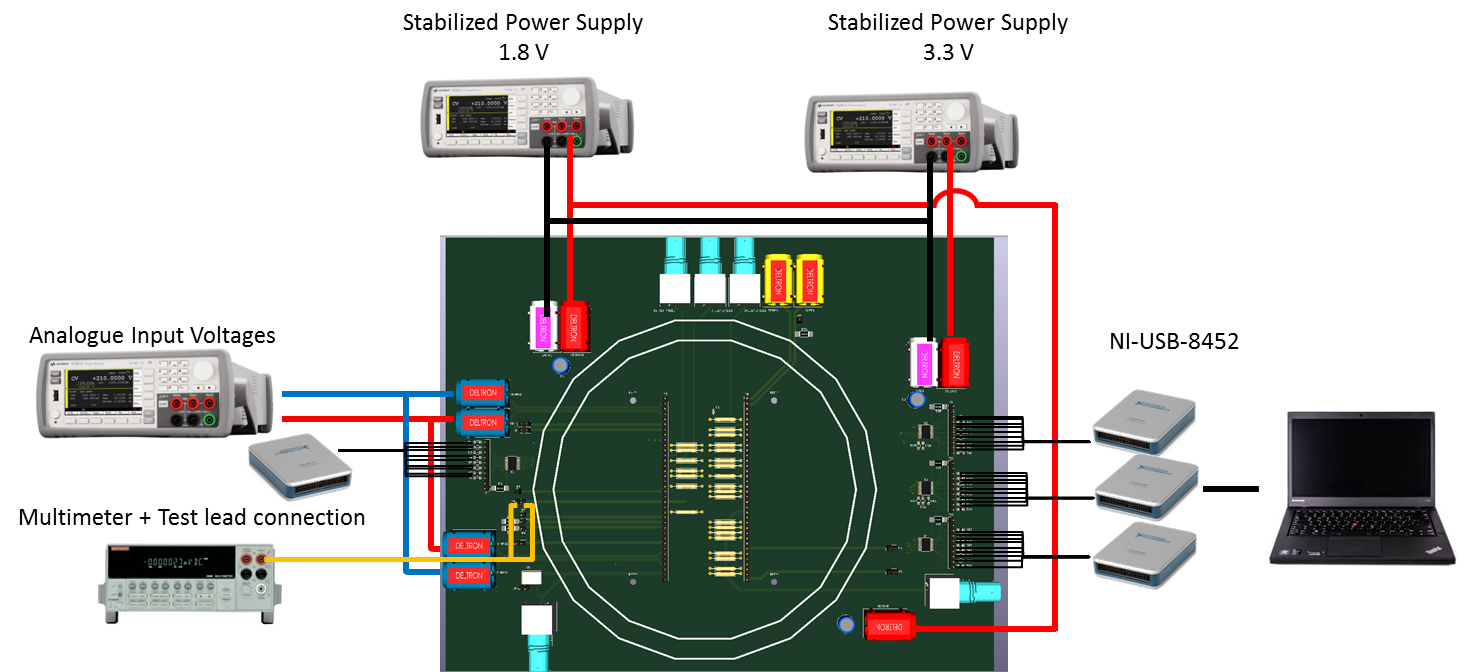
\includegraphics[width=.8\textwidth]{Chapter5/Figs/delay_board_setup.png}
    \caption{Bench-Top installation to measure the delay of comparators}
    \label{fig:doe003_measurebench}
\end{figure}

Either a homemade software or LabView is required to drive the NI-USB boxes. In our case, they are driven by the Labview API provided into a C code, allowing us to drive pins of SPI port as DIO.

For all possible configurations of CALIBN and DLY\_ONLY signals, we measure the frequencies generated for the following temperatures: -40$\degree$C, -25$\degree$C, -10$\degree$C, 0$\degree$C, 27$\degree$C, 85$\degree$C, 100$\degree$C, 125$\degree$C, 150$\degree$C, and 175$\degree$C.

Since by design we fixed the frequency divider to be $N = 64$, the delay is given for DLY\_ONLY = `1' by
\begin{equation}
 T_{delay} = \frac{1}{64} \left(\frac{1}{F_{\rm CLKCMP2}}-\frac{1}{F_{\rm CLKCMP1}} \right)
\end{equation}
And the sum of the delay and the time to reset is given for DLY\_ONLY = `0' by
\begin{equation}
    T_{delay}+T_{reset} = \frac{1}{64} \left(\frac{1}{F_{\rm CLKCMP4}}-\frac{1}{F_{\rm CLKCMP3}} \right)
\end{equation}

\begin{figure}[htp]
    \centering
    %% Creator: Matplotlib, PGF backend
%%
%% To include the figure in your LaTeX document, write
%%   \input{<filename>.pgf}
%%
%% Make sure the required packages are loaded in your preamble
%%   \usepackage{pgf}
%%
%% Figures using additional raster images can only be included by \input if
%% they are in the same directory as the main LaTeX file. For loading figures
%% from other directories you can use the `import` package
%%   \usepackage{import}
%% and then include the figures with
%%   \import{<path to file>}{<filename>.pgf}
%%
%% Matplotlib used the following preamble
%%   \usepackage{gensymb}
%%   \usepackage[utf8x]{inputenc}
%%   \usepackage[T1]{fontenc}
%%
\begingroup%
\makeatletter%
\begin{pgfpicture}%
\pgfpathrectangle{\pgfpointorigin}{\pgfqpoint{3.961700in}{2.962412in}}%
\pgfusepath{use as bounding box, clip}%
\begin{pgfscope}%
\pgfsetbuttcap%
\pgfsetmiterjoin%
\definecolor{currentfill}{rgb}{1.000000,1.000000,1.000000}%
\pgfsetfillcolor{currentfill}%
\pgfsetlinewidth{0.000000pt}%
\definecolor{currentstroke}{rgb}{1.000000,1.000000,1.000000}%
\pgfsetstrokecolor{currentstroke}%
\pgfsetdash{}{0pt}%
\pgfpathmoveto{\pgfqpoint{0.000000in}{0.000000in}}%
\pgfpathlineto{\pgfqpoint{3.961700in}{0.000000in}}%
\pgfpathlineto{\pgfqpoint{3.961700in}{2.962412in}}%
\pgfpathlineto{\pgfqpoint{0.000000in}{2.962412in}}%
\pgfpathclose%
\pgfusepath{fill}%
\end{pgfscope}%
\begin{pgfscope}%
\pgfsetbuttcap%
\pgfsetmiterjoin%
\definecolor{currentfill}{rgb}{1.000000,1.000000,1.000000}%
\pgfsetfillcolor{currentfill}%
\pgfsetlinewidth{0.000000pt}%
\definecolor{currentstroke}{rgb}{0.000000,0.000000,0.000000}%
\pgfsetstrokecolor{currentstroke}%
\pgfsetstrokeopacity{0.000000}%
\pgfsetdash{}{0pt}%
\pgfpathmoveto{\pgfqpoint{0.610776in}{0.489099in}}%
\pgfpathlineto{\pgfqpoint{3.757533in}{0.489099in}}%
\pgfpathlineto{\pgfqpoint{3.757533in}{2.814584in}}%
\pgfpathlineto{\pgfqpoint{0.610776in}{2.814584in}}%
\pgfpathclose%
\pgfusepath{fill}%
\end{pgfscope}%
\begin{pgfscope}%
\pgfsetbuttcap%
\pgfsetroundjoin%
\definecolor{currentfill}{rgb}{0.000000,0.000000,0.000000}%
\pgfsetfillcolor{currentfill}%
\pgfsetlinewidth{0.803000pt}%
\definecolor{currentstroke}{rgb}{0.000000,0.000000,0.000000}%
\pgfsetstrokecolor{currentstroke}%
\pgfsetdash{}{0pt}%
\pgfsys@defobject{currentmarker}{\pgfqpoint{0.000000in}{-0.048611in}}{\pgfqpoint{0.000000in}{0.000000in}}{%
\pgfpathmoveto{\pgfqpoint{0.000000in}{0.000000in}}%
\pgfpathlineto{\pgfqpoint{0.000000in}{-0.048611in}}%
\pgfusepath{stroke,fill}%
}%
\begin{pgfscope}%
\pgfsys@transformshift{0.610776in}{0.489099in}%
\pgfsys@useobject{currentmarker}{}%
\end{pgfscope}%
\end{pgfscope}%
\begin{pgfscope}%
\pgftext[x=0.610776in,y=0.391876in,,top]{\fontsize{10.000000}{12.000000}\selectfont \(\displaystyle -40\)}%
\end{pgfscope}%
\begin{pgfscope}%
\pgfsetbuttcap%
\pgfsetroundjoin%
\definecolor{currentfill}{rgb}{0.000000,0.000000,0.000000}%
\pgfsetfillcolor{currentfill}%
\pgfsetlinewidth{0.803000pt}%
\definecolor{currentstroke}{rgb}{0.000000,0.000000,0.000000}%
\pgfsetstrokecolor{currentstroke}%
\pgfsetdash{}{0pt}%
\pgfsys@defobject{currentmarker}{\pgfqpoint{0.000000in}{-0.048611in}}{\pgfqpoint{0.000000in}{0.000000in}}{%
\pgfpathmoveto{\pgfqpoint{0.000000in}{0.000000in}}%
\pgfpathlineto{\pgfqpoint{0.000000in}{-0.048611in}}%
\pgfusepath{stroke,fill}%
}%
\begin{pgfscope}%
\pgfsys@transformshift{1.196219in}{0.489099in}%
\pgfsys@useobject{currentmarker}{}%
\end{pgfscope}%
\end{pgfscope}%
\begin{pgfscope}%
\pgftext[x=1.196219in,y=0.391876in,,top]{\fontsize{10.000000}{12.000000}\selectfont \(\displaystyle 0\)}%
\end{pgfscope}%
\begin{pgfscope}%
\pgfsetbuttcap%
\pgfsetroundjoin%
\definecolor{currentfill}{rgb}{0.000000,0.000000,0.000000}%
\pgfsetfillcolor{currentfill}%
\pgfsetlinewidth{0.803000pt}%
\definecolor{currentstroke}{rgb}{0.000000,0.000000,0.000000}%
\pgfsetstrokecolor{currentstroke}%
\pgfsetdash{}{0pt}%
\pgfsys@defobject{currentmarker}{\pgfqpoint{0.000000in}{-0.048611in}}{\pgfqpoint{0.000000in}{0.000000in}}{%
\pgfpathmoveto{\pgfqpoint{0.000000in}{0.000000in}}%
\pgfpathlineto{\pgfqpoint{0.000000in}{-0.048611in}}%
\pgfusepath{stroke,fill}%
}%
\begin{pgfscope}%
\pgfsys@transformshift{1.591393in}{0.489099in}%
\pgfsys@useobject{currentmarker}{}%
\end{pgfscope}%
\end{pgfscope}%
\begin{pgfscope}%
\pgftext[x=1.591393in,y=0.391876in,,top]{\fontsize{10.000000}{12.000000}\selectfont \(\displaystyle 27\)}%
\end{pgfscope}%
\begin{pgfscope}%
\pgfsetbuttcap%
\pgfsetroundjoin%
\definecolor{currentfill}{rgb}{0.000000,0.000000,0.000000}%
\pgfsetfillcolor{currentfill}%
\pgfsetlinewidth{0.803000pt}%
\definecolor{currentstroke}{rgb}{0.000000,0.000000,0.000000}%
\pgfsetstrokecolor{currentstroke}%
\pgfsetdash{}{0pt}%
\pgfsys@defobject{currentmarker}{\pgfqpoint{0.000000in}{-0.048611in}}{\pgfqpoint{0.000000in}{0.000000in}}{%
\pgfpathmoveto{\pgfqpoint{0.000000in}{0.000000in}}%
\pgfpathlineto{\pgfqpoint{0.000000in}{-0.048611in}}%
\pgfusepath{stroke,fill}%
}%
\begin{pgfscope}%
\pgfsys@transformshift{2.440286in}{0.489099in}%
\pgfsys@useobject{currentmarker}{}%
\end{pgfscope}%
\end{pgfscope}%
\begin{pgfscope}%
\pgftext[x=2.440286in,y=0.391876in,,top]{\fontsize{10.000000}{12.000000}\selectfont \(\displaystyle 85\)}%
\end{pgfscope}%
\begin{pgfscope}%
\pgfsetbuttcap%
\pgfsetroundjoin%
\definecolor{currentfill}{rgb}{0.000000,0.000000,0.000000}%
\pgfsetfillcolor{currentfill}%
\pgfsetlinewidth{0.803000pt}%
\definecolor{currentstroke}{rgb}{0.000000,0.000000,0.000000}%
\pgfsetstrokecolor{currentstroke}%
\pgfsetdash{}{0pt}%
\pgfsys@defobject{currentmarker}{\pgfqpoint{0.000000in}{-0.048611in}}{\pgfqpoint{0.000000in}{0.000000in}}{%
\pgfpathmoveto{\pgfqpoint{0.000000in}{0.000000in}}%
\pgfpathlineto{\pgfqpoint{0.000000in}{-0.048611in}}%
\pgfusepath{stroke,fill}%
}%
\begin{pgfscope}%
\pgfsys@transformshift{3.391631in}{0.489099in}%
\pgfsys@useobject{currentmarker}{}%
\end{pgfscope}%
\end{pgfscope}%
\begin{pgfscope}%
\pgftext[x=3.391631in,y=0.391876in,,top]{\fontsize{10.000000}{12.000000}\selectfont \(\displaystyle 150\)}%
\end{pgfscope}%
\begin{pgfscope}%
\pgfsetbuttcap%
\pgfsetroundjoin%
\definecolor{currentfill}{rgb}{0.000000,0.000000,0.000000}%
\pgfsetfillcolor{currentfill}%
\pgfsetlinewidth{0.803000pt}%
\definecolor{currentstroke}{rgb}{0.000000,0.000000,0.000000}%
\pgfsetstrokecolor{currentstroke}%
\pgfsetdash{}{0pt}%
\pgfsys@defobject{currentmarker}{\pgfqpoint{0.000000in}{-0.048611in}}{\pgfqpoint{0.000000in}{0.000000in}}{%
\pgfpathmoveto{\pgfqpoint{0.000000in}{0.000000in}}%
\pgfpathlineto{\pgfqpoint{0.000000in}{-0.048611in}}%
\pgfusepath{stroke,fill}%
}%
\begin{pgfscope}%
\pgfsys@transformshift{3.757533in}{0.489099in}%
\pgfsys@useobject{currentmarker}{}%
\end{pgfscope}%
\end{pgfscope}%
\begin{pgfscope}%
\pgftext[x=3.757533in,y=0.391876in,,top]{\fontsize{10.000000}{12.000000}\selectfont \(\displaystyle 175\)}%
\end{pgfscope}%
\begin{pgfscope}%
\pgftext[x=2.184154in,y=0.213666in,,top]{\fontsize{8.000000}{9.600000}\selectfont Temperature [\(\displaystyle \degree\)C]}%
\end{pgfscope}%
\begin{pgfscope}%
\pgfsetbuttcap%
\pgfsetroundjoin%
\definecolor{currentfill}{rgb}{0.000000,0.000000,0.000000}%
\pgfsetfillcolor{currentfill}%
\pgfsetlinewidth{0.803000pt}%
\definecolor{currentstroke}{rgb}{0.000000,0.000000,0.000000}%
\pgfsetstrokecolor{currentstroke}%
\pgfsetdash{}{0pt}%
\pgfsys@defobject{currentmarker}{\pgfqpoint{-0.048611in}{0.000000in}}{\pgfqpoint{0.000000in}{0.000000in}}{%
\pgfpathmoveto{\pgfqpoint{0.000000in}{0.000000in}}%
\pgfpathlineto{\pgfqpoint{-0.048611in}{0.000000in}}%
\pgfusepath{stroke,fill}%
}%
\begin{pgfscope}%
\pgfsys@transformshift{0.610776in}{0.489099in}%
\pgfsys@useobject{currentmarker}{}%
\end{pgfscope}%
\end{pgfscope}%
\begin{pgfscope}%
\pgftext[x=0.266640in,y=0.441271in,left,base]{\fontsize{10.000000}{12.000000}\selectfont \(\displaystyle 1.25\)}%
\end{pgfscope}%
\begin{pgfscope}%
\pgfsetbuttcap%
\pgfsetroundjoin%
\definecolor{currentfill}{rgb}{0.000000,0.000000,0.000000}%
\pgfsetfillcolor{currentfill}%
\pgfsetlinewidth{0.803000pt}%
\definecolor{currentstroke}{rgb}{0.000000,0.000000,0.000000}%
\pgfsetstrokecolor{currentstroke}%
\pgfsetdash{}{0pt}%
\pgfsys@defobject{currentmarker}{\pgfqpoint{-0.048611in}{0.000000in}}{\pgfqpoint{0.000000in}{0.000000in}}{%
\pgfpathmoveto{\pgfqpoint{0.000000in}{0.000000in}}%
\pgfpathlineto{\pgfqpoint{-0.048611in}{0.000000in}}%
\pgfusepath{stroke,fill}%
}%
\begin{pgfscope}%
\pgfsys@transformshift{0.610776in}{1.070470in}%
\pgfsys@useobject{currentmarker}{}%
\end{pgfscope}%
\end{pgfscope}%
\begin{pgfscope}%
\pgftext[x=0.266640in,y=1.022642in,left,base]{\fontsize{10.000000}{12.000000}\selectfont \(\displaystyle 1.50\)}%
\end{pgfscope}%
\begin{pgfscope}%
\pgfsetbuttcap%
\pgfsetroundjoin%
\definecolor{currentfill}{rgb}{0.000000,0.000000,0.000000}%
\pgfsetfillcolor{currentfill}%
\pgfsetlinewidth{0.803000pt}%
\definecolor{currentstroke}{rgb}{0.000000,0.000000,0.000000}%
\pgfsetstrokecolor{currentstroke}%
\pgfsetdash{}{0pt}%
\pgfsys@defobject{currentmarker}{\pgfqpoint{-0.048611in}{0.000000in}}{\pgfqpoint{0.000000in}{0.000000in}}{%
\pgfpathmoveto{\pgfqpoint{0.000000in}{0.000000in}}%
\pgfpathlineto{\pgfqpoint{-0.048611in}{0.000000in}}%
\pgfusepath{stroke,fill}%
}%
\begin{pgfscope}%
\pgfsys@transformshift{0.610776in}{1.651841in}%
\pgfsys@useobject{currentmarker}{}%
\end{pgfscope}%
\end{pgfscope}%
\begin{pgfscope}%
\pgftext[x=0.266640in,y=1.604014in,left,base]{\fontsize{10.000000}{12.000000}\selectfont \(\displaystyle 1.75\)}%
\end{pgfscope}%
\begin{pgfscope}%
\pgfsetbuttcap%
\pgfsetroundjoin%
\definecolor{currentfill}{rgb}{0.000000,0.000000,0.000000}%
\pgfsetfillcolor{currentfill}%
\pgfsetlinewidth{0.803000pt}%
\definecolor{currentstroke}{rgb}{0.000000,0.000000,0.000000}%
\pgfsetstrokecolor{currentstroke}%
\pgfsetdash{}{0pt}%
\pgfsys@defobject{currentmarker}{\pgfqpoint{-0.048611in}{0.000000in}}{\pgfqpoint{0.000000in}{0.000000in}}{%
\pgfpathmoveto{\pgfqpoint{0.000000in}{0.000000in}}%
\pgfpathlineto{\pgfqpoint{-0.048611in}{0.000000in}}%
\pgfusepath{stroke,fill}%
}%
\begin{pgfscope}%
\pgfsys@transformshift{0.610776in}{2.233213in}%
\pgfsys@useobject{currentmarker}{}%
\end{pgfscope}%
\end{pgfscope}%
\begin{pgfscope}%
\pgftext[x=0.266640in,y=2.185385in,left,base]{\fontsize{10.000000}{12.000000}\selectfont \(\displaystyle 2.00\)}%
\end{pgfscope}%
\begin{pgfscope}%
\pgfsetbuttcap%
\pgfsetroundjoin%
\definecolor{currentfill}{rgb}{0.000000,0.000000,0.000000}%
\pgfsetfillcolor{currentfill}%
\pgfsetlinewidth{0.803000pt}%
\definecolor{currentstroke}{rgb}{0.000000,0.000000,0.000000}%
\pgfsetstrokecolor{currentstroke}%
\pgfsetdash{}{0pt}%
\pgfsys@defobject{currentmarker}{\pgfqpoint{-0.048611in}{0.000000in}}{\pgfqpoint{0.000000in}{0.000000in}}{%
\pgfpathmoveto{\pgfqpoint{0.000000in}{0.000000in}}%
\pgfpathlineto{\pgfqpoint{-0.048611in}{0.000000in}}%
\pgfusepath{stroke,fill}%
}%
\begin{pgfscope}%
\pgfsys@transformshift{0.610776in}{2.814584in}%
\pgfsys@useobject{currentmarker}{}%
\end{pgfscope}%
\end{pgfscope}%
\begin{pgfscope}%
\pgftext[x=0.266640in,y=2.766756in,left,base]{\fontsize{10.000000}{12.000000}\selectfont \(\displaystyle 2.25\)}%
\end{pgfscope}%
\begin{pgfscope}%
\pgftext[x=0.211084in,y=1.651841in,,bottom,rotate=90.000000]{\fontsize{8.000000}{9.600000}\selectfont Time Delay [ns]}%
\end{pgfscope}%
\begin{pgfscope}%
\pgfpathrectangle{\pgfqpoint{0.610776in}{0.489099in}}{\pgfqpoint{3.146757in}{2.325486in}} %
\pgfusepath{clip}%
\pgfsetrectcap%
\pgfsetroundjoin%
\pgfsetlinewidth{2.007500pt}%
\definecolor{currentstroke}{rgb}{1.000000,0.000000,0.000000}%
\pgfsetstrokecolor{currentstroke}%
\pgfsetdash{}{0pt}%
\pgfpathmoveto{\pgfqpoint{0.610776in}{0.554069in}}%
\pgfpathlineto{\pgfqpoint{0.830317in}{0.684222in}}%
\pgfpathlineto{\pgfqpoint{1.196219in}{0.895756in}}%
\pgfpathlineto{\pgfqpoint{1.562121in}{1.101127in}}%
\pgfpathlineto{\pgfqpoint{1.591393in}{1.114632in}}%
\pgfpathlineto{\pgfqpoint{2.103656in}{1.389943in}}%
\pgfpathlineto{\pgfqpoint{2.440286in}{1.557671in}}%
\pgfpathlineto{\pgfqpoint{2.659827in}{1.713567in}}%
\pgfpathlineto{\pgfqpoint{3.025729in}{1.907846in}}%
\pgfpathlineto{\pgfqpoint{3.391631in}{2.113404in}}%
\pgfpathlineto{\pgfqpoint{3.757533in}{2.360913in}}%
\pgfusepath{stroke}%
\end{pgfscope}%
\begin{pgfscope}%
\pgfpathrectangle{\pgfqpoint{0.610776in}{0.489099in}}{\pgfqpoint{3.146757in}{2.325486in}} %
\pgfusepath{clip}%
\pgfsetbuttcap%
\pgfsetroundjoin%
\definecolor{currentfill}{rgb}{0.000000,0.000000,0.000000}%
\pgfsetfillcolor{currentfill}%
\pgfsetlinewidth{1.003750pt}%
\definecolor{currentstroke}{rgb}{0.000000,0.000000,0.000000}%
\pgfsetstrokecolor{currentstroke}%
\pgfsetdash{}{0pt}%
\pgfsys@defobject{currentmarker}{\pgfqpoint{-0.020833in}{-0.020833in}}{\pgfqpoint{0.020833in}{0.020833in}}{%
\pgfpathmoveto{\pgfqpoint{0.000000in}{-0.020833in}}%
\pgfpathcurveto{\pgfqpoint{0.005525in}{-0.020833in}}{\pgfqpoint{0.010825in}{-0.018638in}}{\pgfqpoint{0.014731in}{-0.014731in}}%
\pgfpathcurveto{\pgfqpoint{0.018638in}{-0.010825in}}{\pgfqpoint{0.020833in}{-0.005525in}}{\pgfqpoint{0.020833in}{0.000000in}}%
\pgfpathcurveto{\pgfqpoint{0.020833in}{0.005525in}}{\pgfqpoint{0.018638in}{0.010825in}}{\pgfqpoint{0.014731in}{0.014731in}}%
\pgfpathcurveto{\pgfqpoint{0.010825in}{0.018638in}}{\pgfqpoint{0.005525in}{0.020833in}}{\pgfqpoint{0.000000in}{0.020833in}}%
\pgfpathcurveto{\pgfqpoint{-0.005525in}{0.020833in}}{\pgfqpoint{-0.010825in}{0.018638in}}{\pgfqpoint{-0.014731in}{0.014731in}}%
\pgfpathcurveto{\pgfqpoint{-0.018638in}{0.010825in}}{\pgfqpoint{-0.020833in}{0.005525in}}{\pgfqpoint{-0.020833in}{0.000000in}}%
\pgfpathcurveto{\pgfqpoint{-0.020833in}{-0.005525in}}{\pgfqpoint{-0.018638in}{-0.010825in}}{\pgfqpoint{-0.014731in}{-0.014731in}}%
\pgfpathcurveto{\pgfqpoint{-0.010825in}{-0.018638in}}{\pgfqpoint{-0.005525in}{-0.020833in}}{\pgfqpoint{0.000000in}{-0.020833in}}%
\pgfpathclose%
\pgfusepath{stroke,fill}%
}%
\begin{pgfscope}%
\pgfsys@transformshift{0.610776in}{0.520228in}%
\pgfsys@useobject{currentmarker}{}%
\end{pgfscope}%
\begin{pgfscope}%
\pgfsys@transformshift{0.830317in}{0.632491in}%
\pgfsys@useobject{currentmarker}{}%
\end{pgfscope}%
\begin{pgfscope}%
\pgfsys@transformshift{1.196219in}{0.810982in}%
\pgfsys@useobject{currentmarker}{}%
\end{pgfscope}%
\begin{pgfscope}%
\pgfsys@transformshift{1.562121in}{0.966724in}%
\pgfsys@useobject{currentmarker}{}%
\end{pgfscope}%
\begin{pgfscope}%
\pgfsys@transformshift{1.576757in}{0.978761in}%
\pgfsys@useobject{currentmarker}{}%
\end{pgfscope}%
\begin{pgfscope}%
\pgfsys@transformshift{1.591393in}{0.977679in}%
\pgfsys@useobject{currentmarker}{}%
\end{pgfscope}%
\begin{pgfscope}%
\pgfsys@transformshift{1.598711in}{0.993676in}%
\pgfsys@useobject{currentmarker}{}%
\end{pgfscope}%
\begin{pgfscope}%
\pgfsys@transformshift{1.928023in}{1.192563in}%
\pgfsys@useobject{currentmarker}{}%
\end{pgfscope}%
\begin{pgfscope}%
\pgfsys@transformshift{2.367105in}{1.444402in}%
\pgfsys@useobject{currentmarker}{}%
\end{pgfscope}%
\begin{pgfscope}%
\pgfsys@transformshift{2.659827in}{1.644734in}%
\pgfsys@useobject{currentmarker}{}%
\end{pgfscope}%
\begin{pgfscope}%
\pgfsys@transformshift{3.025729in}{1.881437in}%
\pgfsys@useobject{currentmarker}{}%
\end{pgfscope}%
\begin{pgfscope}%
\pgfsys@transformshift{3.245270in}{2.028786in}%
\pgfsys@useobject{currentmarker}{}%
\end{pgfscope}%
\begin{pgfscope}%
\pgfsys@transformshift{3.391631in}{2.135870in}%
\pgfsys@useobject{currentmarker}{}%
\end{pgfscope}%
\begin{pgfscope}%
\pgfsys@transformshift{3.537991in}{2.242192in}%
\pgfsys@useobject{currentmarker}{}%
\end{pgfscope}%
\begin{pgfscope}%
\pgfsys@transformshift{3.684352in}{2.348776in}%
\pgfsys@useobject{currentmarker}{}%
\end{pgfscope}%
\begin{pgfscope}%
\pgfsys@transformshift{3.757533in}{2.398322in}%
\pgfsys@useobject{currentmarker}{}%
\end{pgfscope}%
\end{pgfscope}%
\begin{pgfscope}%
\pgfpathrectangle{\pgfqpoint{0.610776in}{0.489099in}}{\pgfqpoint{3.146757in}{2.325486in}} %
\pgfusepath{clip}%
\pgfsetbuttcap%
\pgfsetroundjoin%
\definecolor{currentfill}{rgb}{0.000000,0.500000,0.000000}%
\pgfsetfillcolor{currentfill}%
\pgfsetlinewidth{1.003750pt}%
\definecolor{currentstroke}{rgb}{0.000000,0.500000,0.000000}%
\pgfsetstrokecolor{currentstroke}%
\pgfsetdash{}{0pt}%
\pgfsys@defobject{currentmarker}{\pgfqpoint{-0.020833in}{-0.020833in}}{\pgfqpoint{0.020833in}{0.020833in}}{%
\pgfpathmoveto{\pgfqpoint{0.000000in}{-0.020833in}}%
\pgfpathcurveto{\pgfqpoint{0.005525in}{-0.020833in}}{\pgfqpoint{0.010825in}{-0.018638in}}{\pgfqpoint{0.014731in}{-0.014731in}}%
\pgfpathcurveto{\pgfqpoint{0.018638in}{-0.010825in}}{\pgfqpoint{0.020833in}{-0.005525in}}{\pgfqpoint{0.020833in}{0.000000in}}%
\pgfpathcurveto{\pgfqpoint{0.020833in}{0.005525in}}{\pgfqpoint{0.018638in}{0.010825in}}{\pgfqpoint{0.014731in}{0.014731in}}%
\pgfpathcurveto{\pgfqpoint{0.010825in}{0.018638in}}{\pgfqpoint{0.005525in}{0.020833in}}{\pgfqpoint{0.000000in}{0.020833in}}%
\pgfpathcurveto{\pgfqpoint{-0.005525in}{0.020833in}}{\pgfqpoint{-0.010825in}{0.018638in}}{\pgfqpoint{-0.014731in}{0.014731in}}%
\pgfpathcurveto{\pgfqpoint{-0.018638in}{0.010825in}}{\pgfqpoint{-0.020833in}{0.005525in}}{\pgfqpoint{-0.020833in}{0.000000in}}%
\pgfpathcurveto{\pgfqpoint{-0.020833in}{-0.005525in}}{\pgfqpoint{-0.018638in}{-0.010825in}}{\pgfqpoint{-0.014731in}{-0.014731in}}%
\pgfpathcurveto{\pgfqpoint{-0.010825in}{-0.018638in}}{\pgfqpoint{-0.005525in}{-0.020833in}}{\pgfqpoint{0.000000in}{-0.020833in}}%
\pgfpathclose%
\pgfusepath{stroke,fill}%
}%
\begin{pgfscope}%
\pgfsys@transformshift{0.610776in}{0.631593in}%
\pgfsys@useobject{currentmarker}{}%
\end{pgfscope}%
\begin{pgfscope}%
\pgfsys@transformshift{0.757137in}{0.713028in}%
\pgfsys@useobject{currentmarker}{}%
\end{pgfscope}%
\begin{pgfscope}%
\pgfsys@transformshift{0.830317in}{0.768294in}%
\pgfsys@useobject{currentmarker}{}%
\end{pgfscope}%
\begin{pgfscope}%
\pgfsys@transformshift{0.903498in}{0.802436in}%
\pgfsys@useobject{currentmarker}{}%
\end{pgfscope}%
\begin{pgfscope}%
\pgfsys@transformshift{1.049858in}{0.795605in}%
\pgfsys@useobject{currentmarker}{}%
\end{pgfscope}%
\begin{pgfscope}%
\pgfsys@transformshift{1.196219in}{0.870740in}%
\pgfsys@useobject{currentmarker}{}%
\end{pgfscope}%
\begin{pgfscope}%
\pgfsys@transformshift{1.342580in}{0.952263in}%
\pgfsys@useobject{currentmarker}{}%
\end{pgfscope}%
\begin{pgfscope}%
\pgfsys@transformshift{1.488941in}{1.054454in}%
\pgfsys@useobject{currentmarker}{}%
\end{pgfscope}%
\begin{pgfscope}%
\pgfsys@transformshift{1.562121in}{1.080085in}%
\pgfsys@useobject{currentmarker}{}%
\end{pgfscope}%
\begin{pgfscope}%
\pgfsys@transformshift{1.591393in}{1.155207in}%
\pgfsys@useobject{currentmarker}{}%
\end{pgfscope}%
\begin{pgfscope}%
\pgfsys@transformshift{1.598711in}{0.975990in}%
\pgfsys@useobject{currentmarker}{}%
\end{pgfscope}%
\begin{pgfscope}%
\pgfsys@transformshift{1.635301in}{1.133599in}%
\pgfsys@useobject{currentmarker}{}%
\end{pgfscope}%
\begin{pgfscope}%
\pgfsys@transformshift{1.781662in}{1.222368in}%
\pgfsys@useobject{currentmarker}{}%
\end{pgfscope}%
\begin{pgfscope}%
\pgfsys@transformshift{1.928023in}{1.303555in}%
\pgfsys@useobject{currentmarker}{}%
\end{pgfscope}%
\begin{pgfscope}%
\pgfsys@transformshift{2.074384in}{1.409265in}%
\pgfsys@useobject{currentmarker}{}%
\end{pgfscope}%
\begin{pgfscope}%
\pgfsys@transformshift{2.220745in}{1.488263in}%
\pgfsys@useobject{currentmarker}{}%
\end{pgfscope}%
\begin{pgfscope}%
\pgfsys@transformshift{2.367105in}{1.590297in}%
\pgfsys@useobject{currentmarker}{}%
\end{pgfscope}%
\begin{pgfscope}%
\pgfsys@transformshift{2.513466in}{1.673493in}%
\pgfsys@useobject{currentmarker}{}%
\end{pgfscope}%
\begin{pgfscope}%
\pgfsys@transformshift{2.659827in}{1.778264in}%
\pgfsys@useobject{currentmarker}{}%
\end{pgfscope}%
\begin{pgfscope}%
\pgfsys@transformshift{2.806188in}{1.770412in}%
\pgfsys@useobject{currentmarker}{}%
\end{pgfscope}%
\begin{pgfscope}%
\pgfsys@transformshift{2.952548in}{1.864897in}%
\pgfsys@useobject{currentmarker}{}%
\end{pgfscope}%
\begin{pgfscope}%
\pgfsys@transformshift{3.025729in}{1.915040in}%
\pgfsys@useobject{currentmarker}{}%
\end{pgfscope}%
\begin{pgfscope}%
\pgfsys@transformshift{3.098909in}{1.964185in}%
\pgfsys@useobject{currentmarker}{}%
\end{pgfscope}%
\begin{pgfscope}%
\pgfsys@transformshift{3.245270in}{2.070006in}%
\pgfsys@useobject{currentmarker}{}%
\end{pgfscope}%
\begin{pgfscope}%
\pgfsys@transformshift{3.391631in}{2.172868in}%
\pgfsys@useobject{currentmarker}{}%
\end{pgfscope}%
\begin{pgfscope}%
\pgfsys@transformshift{3.537991in}{2.275951in}%
\pgfsys@useobject{currentmarker}{}%
\end{pgfscope}%
\begin{pgfscope}%
\pgfsys@transformshift{3.684352in}{2.388773in}%
\pgfsys@useobject{currentmarker}{}%
\end{pgfscope}%
\begin{pgfscope}%
\pgfsys@transformshift{3.757533in}{2.458560in}%
\pgfsys@useobject{currentmarker}{}%
\end{pgfscope}%
\end{pgfscope}%
\begin{pgfscope}%
\pgfpathrectangle{\pgfqpoint{0.610776in}{0.489099in}}{\pgfqpoint{3.146757in}{2.325486in}} %
\pgfusepath{clip}%
\pgfsetbuttcap%
\pgfsetroundjoin%
\definecolor{currentfill}{rgb}{0.000000,0.000000,1.000000}%
\pgfsetfillcolor{currentfill}%
\pgfsetlinewidth{1.003750pt}%
\definecolor{currentstroke}{rgb}{0.000000,0.000000,1.000000}%
\pgfsetstrokecolor{currentstroke}%
\pgfsetdash{}{0pt}%
\pgfsys@defobject{currentmarker}{\pgfqpoint{-0.020833in}{-0.020833in}}{\pgfqpoint{0.020833in}{0.020833in}}{%
\pgfpathmoveto{\pgfqpoint{0.000000in}{-0.020833in}}%
\pgfpathcurveto{\pgfqpoint{0.005525in}{-0.020833in}}{\pgfqpoint{0.010825in}{-0.018638in}}{\pgfqpoint{0.014731in}{-0.014731in}}%
\pgfpathcurveto{\pgfqpoint{0.018638in}{-0.010825in}}{\pgfqpoint{0.020833in}{-0.005525in}}{\pgfqpoint{0.020833in}{0.000000in}}%
\pgfpathcurveto{\pgfqpoint{0.020833in}{0.005525in}}{\pgfqpoint{0.018638in}{0.010825in}}{\pgfqpoint{0.014731in}{0.014731in}}%
\pgfpathcurveto{\pgfqpoint{0.010825in}{0.018638in}}{\pgfqpoint{0.005525in}{0.020833in}}{\pgfqpoint{0.000000in}{0.020833in}}%
\pgfpathcurveto{\pgfqpoint{-0.005525in}{0.020833in}}{\pgfqpoint{-0.010825in}{0.018638in}}{\pgfqpoint{-0.014731in}{0.014731in}}%
\pgfpathcurveto{\pgfqpoint{-0.018638in}{0.010825in}}{\pgfqpoint{-0.020833in}{0.005525in}}{\pgfqpoint{-0.020833in}{0.000000in}}%
\pgfpathcurveto{\pgfqpoint{-0.020833in}{-0.005525in}}{\pgfqpoint{-0.018638in}{-0.010825in}}{\pgfqpoint{-0.014731in}{-0.014731in}}%
\pgfpathcurveto{\pgfqpoint{-0.010825in}{-0.018638in}}{\pgfqpoint{-0.005525in}{-0.020833in}}{\pgfqpoint{0.000000in}{-0.020833in}}%
\pgfpathclose%
\pgfusepath{stroke,fill}%
}%
\begin{pgfscope}%
\pgfsys@transformshift{0.610776in}{0.587210in}%
\pgfsys@useobject{currentmarker}{}%
\end{pgfscope}%
\begin{pgfscope}%
\pgfsys@transformshift{0.830317in}{0.732885in}%
\pgfsys@useobject{currentmarker}{}%
\end{pgfscope}%
\begin{pgfscope}%
\pgfsys@transformshift{1.196219in}{0.927831in}%
\pgfsys@useobject{currentmarker}{}%
\end{pgfscope}%
\begin{pgfscope}%
\pgfsys@transformshift{1.562121in}{1.080683in}%
\pgfsys@useobject{currentmarker}{}%
\end{pgfscope}%
\begin{pgfscope}%
\pgfsys@transformshift{1.591393in}{1.110380in}%
\pgfsys@useobject{currentmarker}{}%
\end{pgfscope}%
\begin{pgfscope}%
\pgfsys@transformshift{1.598711in}{1.122384in}%
\pgfsys@useobject{currentmarker}{}%
\end{pgfscope}%
\begin{pgfscope}%
\pgfsys@transformshift{1.928023in}{1.330417in}%
\pgfsys@useobject{currentmarker}{}%
\end{pgfscope}%
\begin{pgfscope}%
\pgfsys@transformshift{2.367105in}{1.573417in}%
\pgfsys@useobject{currentmarker}{}%
\end{pgfscope}%
\begin{pgfscope}%
\pgfsys@transformshift{2.659827in}{1.795402in}%
\pgfsys@useobject{currentmarker}{}%
\end{pgfscope}%
\begin{pgfscope}%
\pgfsys@transformshift{3.025729in}{1.893013in}%
\pgfsys@useobject{currentmarker}{}%
\end{pgfscope}%
\begin{pgfscope}%
\pgfsys@transformshift{3.245270in}{2.068597in}%
\pgfsys@useobject{currentmarker}{}%
\end{pgfscope}%
\begin{pgfscope}%
\pgfsys@transformshift{3.391631in}{2.160189in}%
\pgfsys@useobject{currentmarker}{}%
\end{pgfscope}%
\begin{pgfscope}%
\pgfsys@transformshift{3.537991in}{2.294410in}%
\pgfsys@useobject{currentmarker}{}%
\end{pgfscope}%
\begin{pgfscope}%
\pgfsys@transformshift{3.684352in}{2.394205in}%
\pgfsys@useobject{currentmarker}{}%
\end{pgfscope}%
\begin{pgfscope}%
\pgfsys@transformshift{3.757533in}{2.532729in}%
\pgfsys@useobject{currentmarker}{}%
\end{pgfscope}%
\end{pgfscope}%
\begin{pgfscope}%
\pgfsetrectcap%
\pgfsetmiterjoin%
\pgfsetlinewidth{0.803000pt}%
\definecolor{currentstroke}{rgb}{0.000000,0.000000,0.000000}%
\pgfsetstrokecolor{currentstroke}%
\pgfsetdash{}{0pt}%
\pgfpathmoveto{\pgfqpoint{0.610776in}{0.489099in}}%
\pgfpathlineto{\pgfqpoint{0.610776in}{2.814584in}}%
\pgfusepath{stroke}%
\end{pgfscope}%
\begin{pgfscope}%
\pgfsetrectcap%
\pgfsetmiterjoin%
\pgfsetlinewidth{0.803000pt}%
\definecolor{currentstroke}{rgb}{0.000000,0.000000,0.000000}%
\pgfsetstrokecolor{currentstroke}%
\pgfsetdash{}{0pt}%
\pgfpathmoveto{\pgfqpoint{3.757533in}{0.489099in}}%
\pgfpathlineto{\pgfqpoint{3.757533in}{2.814584in}}%
\pgfusepath{stroke}%
\end{pgfscope}%
\begin{pgfscope}%
\pgfsetrectcap%
\pgfsetmiterjoin%
\pgfsetlinewidth{0.803000pt}%
\definecolor{currentstroke}{rgb}{0.000000,0.000000,0.000000}%
\pgfsetstrokecolor{currentstroke}%
\pgfsetdash{}{0pt}%
\pgfpathmoveto{\pgfqpoint{0.610776in}{0.489099in}}%
\pgfpathlineto{\pgfqpoint{3.757533in}{0.489099in}}%
\pgfusepath{stroke}%
\end{pgfscope}%
\begin{pgfscope}%
\pgfsetrectcap%
\pgfsetmiterjoin%
\pgfsetlinewidth{0.803000pt}%
\definecolor{currentstroke}{rgb}{0.000000,0.000000,0.000000}%
\pgfsetstrokecolor{currentstroke}%
\pgfsetdash{}{0pt}%
\pgfpathmoveto{\pgfqpoint{0.610776in}{2.814584in}}%
\pgfpathlineto{\pgfqpoint{3.757533in}{2.814584in}}%
\pgfusepath{stroke}%
\end{pgfscope}%
\begin{pgfscope}%
\pgfsetbuttcap%
\pgfsetmiterjoin%
\definecolor{currentfill}{rgb}{1.000000,1.000000,1.000000}%
\pgfsetfillcolor{currentfill}%
\pgfsetfillopacity{0.800000}%
\pgfsetlinewidth{1.003750pt}%
\definecolor{currentstroke}{rgb}{0.800000,0.800000,0.800000}%
\pgfsetstrokecolor{currentstroke}%
\pgfsetstrokeopacity{0.800000}%
\pgfsetdash{}{0pt}%
\pgfpathmoveto{\pgfqpoint{0.707998in}{1.928808in}}%
\pgfpathlineto{\pgfqpoint{2.392495in}{1.928808in}}%
\pgfpathquadraticcurveto{\pgfqpoint{2.420273in}{1.928808in}}{\pgfqpoint{2.420273in}{1.956586in}}%
\pgfpathlineto{\pgfqpoint{2.420273in}{2.717362in}}%
\pgfpathquadraticcurveto{\pgfqpoint{2.420273in}{2.745140in}}{\pgfqpoint{2.392495in}{2.745140in}}%
\pgfpathlineto{\pgfqpoint{0.707998in}{2.745140in}}%
\pgfpathquadraticcurveto{\pgfqpoint{0.680221in}{2.745140in}}{\pgfqpoint{0.680221in}{2.717362in}}%
\pgfpathlineto{\pgfqpoint{0.680221in}{1.956586in}}%
\pgfpathquadraticcurveto{\pgfqpoint{0.680221in}{1.928808in}}{\pgfqpoint{0.707998in}{1.928808in}}%
\pgfpathclose%
\pgfusepath{stroke,fill}%
\end{pgfscope}%
\begin{pgfscope}%
\pgfsetrectcap%
\pgfsetroundjoin%
\pgfsetlinewidth{2.007500pt}%
\definecolor{currentstroke}{rgb}{1.000000,0.000000,0.000000}%
\pgfsetstrokecolor{currentstroke}%
\pgfsetdash{}{0pt}%
\pgfpathmoveto{\pgfqpoint{0.735776in}{2.640973in}}%
\pgfpathlineto{\pgfqpoint{1.013554in}{2.640973in}}%
\pgfusepath{stroke}%
\end{pgfscope}%
\begin{pgfscope}%
\pgftext[x=1.124665in,y=2.592362in,left,base]{\fontsize{10.000000}{12.000000}\selectfont Post-Layout}%
\end{pgfscope}%
\begin{pgfscope}%
\pgfsetbuttcap%
\pgfsetroundjoin%
\definecolor{currentfill}{rgb}{0.000000,0.000000,0.000000}%
\pgfsetfillcolor{currentfill}%
\pgfsetlinewidth{1.003750pt}%
\definecolor{currentstroke}{rgb}{0.000000,0.000000,0.000000}%
\pgfsetstrokecolor{currentstroke}%
\pgfsetdash{}{0pt}%
\pgfsys@defobject{currentmarker}{\pgfqpoint{-0.020833in}{-0.020833in}}{\pgfqpoint{0.020833in}{0.020833in}}{%
\pgfpathmoveto{\pgfqpoint{0.000000in}{-0.020833in}}%
\pgfpathcurveto{\pgfqpoint{0.005525in}{-0.020833in}}{\pgfqpoint{0.010825in}{-0.018638in}}{\pgfqpoint{0.014731in}{-0.014731in}}%
\pgfpathcurveto{\pgfqpoint{0.018638in}{-0.010825in}}{\pgfqpoint{0.020833in}{-0.005525in}}{\pgfqpoint{0.020833in}{0.000000in}}%
\pgfpathcurveto{\pgfqpoint{0.020833in}{0.005525in}}{\pgfqpoint{0.018638in}{0.010825in}}{\pgfqpoint{0.014731in}{0.014731in}}%
\pgfpathcurveto{\pgfqpoint{0.010825in}{0.018638in}}{\pgfqpoint{0.005525in}{0.020833in}}{\pgfqpoint{0.000000in}{0.020833in}}%
\pgfpathcurveto{\pgfqpoint{-0.005525in}{0.020833in}}{\pgfqpoint{-0.010825in}{0.018638in}}{\pgfqpoint{-0.014731in}{0.014731in}}%
\pgfpathcurveto{\pgfqpoint{-0.018638in}{0.010825in}}{\pgfqpoint{-0.020833in}{0.005525in}}{\pgfqpoint{-0.020833in}{0.000000in}}%
\pgfpathcurveto{\pgfqpoint{-0.020833in}{-0.005525in}}{\pgfqpoint{-0.018638in}{-0.010825in}}{\pgfqpoint{-0.014731in}{-0.014731in}}%
\pgfpathcurveto{\pgfqpoint{-0.010825in}{-0.018638in}}{\pgfqpoint{-0.005525in}{-0.020833in}}{\pgfqpoint{0.000000in}{-0.020833in}}%
\pgfpathclose%
\pgfusepath{stroke,fill}%
}%
\begin{pgfscope}%
\pgfsys@transformshift{0.874665in}{2.447307in}%
\pgfsys@useobject{currentmarker}{}%
\end{pgfscope}%
\end{pgfscope}%
\begin{pgfscope}%
\pgftext[x=1.124665in,y=2.398696in,left,base]{\fontsize{10.000000}{12.000000}\selectfont Measures DOE03-13}%
\end{pgfscope}%
\begin{pgfscope}%
\pgfsetbuttcap%
\pgfsetroundjoin%
\definecolor{currentfill}{rgb}{0.000000,0.500000,0.000000}%
\pgfsetfillcolor{currentfill}%
\pgfsetlinewidth{1.003750pt}%
\definecolor{currentstroke}{rgb}{0.000000,0.500000,0.000000}%
\pgfsetstrokecolor{currentstroke}%
\pgfsetdash{}{0pt}%
\pgfsys@defobject{currentmarker}{\pgfqpoint{-0.020833in}{-0.020833in}}{\pgfqpoint{0.020833in}{0.020833in}}{%
\pgfpathmoveto{\pgfqpoint{0.000000in}{-0.020833in}}%
\pgfpathcurveto{\pgfqpoint{0.005525in}{-0.020833in}}{\pgfqpoint{0.010825in}{-0.018638in}}{\pgfqpoint{0.014731in}{-0.014731in}}%
\pgfpathcurveto{\pgfqpoint{0.018638in}{-0.010825in}}{\pgfqpoint{0.020833in}{-0.005525in}}{\pgfqpoint{0.020833in}{0.000000in}}%
\pgfpathcurveto{\pgfqpoint{0.020833in}{0.005525in}}{\pgfqpoint{0.018638in}{0.010825in}}{\pgfqpoint{0.014731in}{0.014731in}}%
\pgfpathcurveto{\pgfqpoint{0.010825in}{0.018638in}}{\pgfqpoint{0.005525in}{0.020833in}}{\pgfqpoint{0.000000in}{0.020833in}}%
\pgfpathcurveto{\pgfqpoint{-0.005525in}{0.020833in}}{\pgfqpoint{-0.010825in}{0.018638in}}{\pgfqpoint{-0.014731in}{0.014731in}}%
\pgfpathcurveto{\pgfqpoint{-0.018638in}{0.010825in}}{\pgfqpoint{-0.020833in}{0.005525in}}{\pgfqpoint{-0.020833in}{0.000000in}}%
\pgfpathcurveto{\pgfqpoint{-0.020833in}{-0.005525in}}{\pgfqpoint{-0.018638in}{-0.010825in}}{\pgfqpoint{-0.014731in}{-0.014731in}}%
\pgfpathcurveto{\pgfqpoint{-0.010825in}{-0.018638in}}{\pgfqpoint{-0.005525in}{-0.020833in}}{\pgfqpoint{0.000000in}{-0.020833in}}%
\pgfpathclose%
\pgfusepath{stroke,fill}%
}%
\begin{pgfscope}%
\pgfsys@transformshift{0.874665in}{2.253641in}%
\pgfsys@useobject{currentmarker}{}%
\end{pgfscope}%
\end{pgfscope}%
\begin{pgfscope}%
\pgftext[x=1.124665in,y=2.205029in,left,base]{\fontsize{10.000000}{12.000000}\selectfont Measures DOE03-15}%
\end{pgfscope}%
\begin{pgfscope}%
\pgfsetbuttcap%
\pgfsetroundjoin%
\definecolor{currentfill}{rgb}{0.000000,0.000000,1.000000}%
\pgfsetfillcolor{currentfill}%
\pgfsetlinewidth{1.003750pt}%
\definecolor{currentstroke}{rgb}{0.000000,0.000000,1.000000}%
\pgfsetstrokecolor{currentstroke}%
\pgfsetdash{}{0pt}%
\pgfsys@defobject{currentmarker}{\pgfqpoint{-0.020833in}{-0.020833in}}{\pgfqpoint{0.020833in}{0.020833in}}{%
\pgfpathmoveto{\pgfqpoint{0.000000in}{-0.020833in}}%
\pgfpathcurveto{\pgfqpoint{0.005525in}{-0.020833in}}{\pgfqpoint{0.010825in}{-0.018638in}}{\pgfqpoint{0.014731in}{-0.014731in}}%
\pgfpathcurveto{\pgfqpoint{0.018638in}{-0.010825in}}{\pgfqpoint{0.020833in}{-0.005525in}}{\pgfqpoint{0.020833in}{0.000000in}}%
\pgfpathcurveto{\pgfqpoint{0.020833in}{0.005525in}}{\pgfqpoint{0.018638in}{0.010825in}}{\pgfqpoint{0.014731in}{0.014731in}}%
\pgfpathcurveto{\pgfqpoint{0.010825in}{0.018638in}}{\pgfqpoint{0.005525in}{0.020833in}}{\pgfqpoint{0.000000in}{0.020833in}}%
\pgfpathcurveto{\pgfqpoint{-0.005525in}{0.020833in}}{\pgfqpoint{-0.010825in}{0.018638in}}{\pgfqpoint{-0.014731in}{0.014731in}}%
\pgfpathcurveto{\pgfqpoint{-0.018638in}{0.010825in}}{\pgfqpoint{-0.020833in}{0.005525in}}{\pgfqpoint{-0.020833in}{0.000000in}}%
\pgfpathcurveto{\pgfqpoint{-0.020833in}{-0.005525in}}{\pgfqpoint{-0.018638in}{-0.010825in}}{\pgfqpoint{-0.014731in}{-0.014731in}}%
\pgfpathcurveto{\pgfqpoint{-0.010825in}{-0.018638in}}{\pgfqpoint{-0.005525in}{-0.020833in}}{\pgfqpoint{0.000000in}{-0.020833in}}%
\pgfpathclose%
\pgfusepath{stroke,fill}%
}%
\begin{pgfscope}%
\pgfsys@transformshift{0.874665in}{2.059974in}%
\pgfsys@useobject{currentmarker}{}%
\end{pgfscope}%
\end{pgfscope}%
\begin{pgfscope}%
\pgftext[x=1.124665in,y=2.011363in,left,base]{\fontsize{10.000000}{12.000000}\selectfont Measures DOE03-19}%
\end{pgfscope}%
\end{pgfpicture}%
\makeatother%
\endgroup%

    \caption{Post-layout delay results versus the estimated delay from the new proposed circuit}
    \label{fig:delay_vs_meas}
\end{figure}

\figurename~\ref{fig:delay_vs_meas} represents the post-layout simulation results of the delay against the measurements results of the new delay estimation circuit for three different samples. We notice that first, the delay after extraction of parasitics is superior to measured values. This can be explained by three main reasons. First, the transistor in the process from which samples are coming from can be more doped than the typical case. Second, the voltage which trigger cells in the circuit is not the same level as the logic level used in the Section~\ref{sec:latches_sim}. And third, a 5 kHz inaccuracy while measuring the delay generate a systematic error of 13 ps for an output frequency around 2.5 MHz.

From sample to sample, we experiment an error which varies from less than 10 ps to 107 ps in the worst case, at 175\(\degree\)C which correspond to an inaccuracy of 25 kHz. Or in other terms, an error of 1\% on the frequency. Despite that, the circuit provides results with an absolute maximum error of 60 ps without correction.

% table comparing area, temperature range, resolution, measurement range, power of solutions listed
Then, the proposed delay measurement circuit is compared to existing circuits to measure the delay of analog component. The comparison in Table~\ref{tbl:delay-measurement-comparison} highlights the small footprint of the proposed solution for a resolution in the order of few picoseconds which compete with traditional Time-to-Digital converter (TDC). Moreover, the proposed circuit achieves the best power consumption known. Nevertheless, toggling at very high frequency induces large transient peaks detected up to 1 mA. 

\renewcommand*{\thefootnote}{\fnsymbol{footnote}}
\begin{table}[htp]
    \centering
    \caption{Comparison of delay measurement circuits}
    \label{tbl:delay-measurement-comparison}
    \begin{tabular}{@{}llllllll@{}}
    \toprule
                                      & \cite{1637593} & \cite{6233014} & \cite{7312496} & \cite{7560219} &  &  & \textbf{proposed} \\ \midrule
    technology  [nm]                  & 350         & 40          & 350        & 65        &  &  & 180              \\
    area [\(\mu m \times \mu m\)]     & 2500 $\times$ 3000 & 1000 $\times$ 300  & 610000     & 120 $\times$ 130 &  &  & 40 $\times$ 30           \\
    resolution [ps]                   & 12.2        & 100         & 0.61       & 2         &  &  & 5\footnotemark                 \\
    max error [ps]                    & 13          & 50          & 4.5        & 3.5       &  &  & 60             \\
    measurement range [\(\mu\)s]      & 202         & 0.003       & 327        & NC        &  &  & NA             \\
    temperature range [\(\degree \)C] & -40 -- +60  & -40 -- +125 & -30 -- +70 & 0 -- +100 &  &  & -40 -- +175       \\
    power consumption [mW]            & 40          & NC          & 80         & 0.78      &  &  & 0.52              \\ \bottomrule
    \end{tabular}
\end{table}

\footnotetext{the resolution of the circuit depends on the resolution of the frequency meter. The resolution given corresponds to the a frequency divider of 64 and a frequency meter able to differentiate 6.01 MHz and 6 MHz}
\renewcommand*{\thefootnote}{\arabic{footnote}}
\setcounter{footnote}{0}

Measurements results confirm the operation of the proposed delay measurement circuit. With a reduced power consumption and a small area overhead, this circuit is well suited for advanced on-chip assessment of comparators over a large temperature range. This circuit has the potential to estimate the offset as the input voltage difference for which the delay measured is the greatest. Furthermore, the measurement is expected to be only limited by the external frequency meter. Besides that, more accurate delay results could only be achieved with a TDC\@. And this circuit is surely a source of noise and EMC near sensitive components.